%!TEX root = these.tex

\chapter{Évaluation hors ligne de formules LTL avec les manipulations de bitmaps}

Ce chapitre présente une version modifiée et traduite d'un article qui est écrit par K. Xie et S. Hallé et qui est encore en cours de révision pour sa publication dans les actes de la conférence internationale: Runtime Verification 2016 (RV'16) à Madrid, Espagne en 2016.

%% ------------------
%% Section: intro
%% ------------------
\section{Introduction}\label{sec:bm:intro} %% {{{

Une \emph{logique temporelle} \citep{huth2004} est un système logistique qui utilise des règles et des symboles pour décrire et raisonner sur le changement de l'état d'un système en termes de temps. Elle est basée sur l'idée qu'un état ne peut pas rester constamment vrai ou faux avec le temps. Une \emph{Logique Temporelle Linéaire (LTL)} \citep{pnueli97} est une logique temporelle, et comme son nom l'implique, une \emph{LTL} peut désigner une seule séquence d'états et pour chaque état il n'y a qu'un état futur.

Un \emph{bitmap}, qui est également connu sous forme de tableau de bites ou de bitset, est une structure compacte de données stockant une séquence de valeurs binaires. Comme on le verra dans la section \ref{sec:bm:compression}, il peut être utilisé pour exprimer un ensemble de nombres, ou un tableau dont chaque bit représente une option de 2 valeurs. Les bitmaps présentent plusieurs avantages en tant qu'une structure de données: ils peuvent représenter brièvement de l'information et fournir des fonctions très efficaces pour les manipuler, grâce au fait que les bits multiples peuvent être traités en parallèle à travers une seule instruction du processeur.

Dans ce chapitre, nous explorons l'idée de l'utilisation des manipulations de bitmaps pour l'évaluation hors ligne de formules LTL d'un journal d'événements. A cet effet, dans la section \ref{sec:bm:ltlbitmap}, nous introduisons une solution qui, pour une trace d'événements données $\sigma$ et une formule LTL $\varphi$, convertit d'abord des termes de base en autant de bitmaps; intuitivement, le bitmap correspondant à une proposition atomique $p$ décrit les événements de $\sigma$ qui satisfont $p$. Les algorithmes sont ensuite détaillés pour chaque opérateur LTL qui prend des bitmaps comme leur entrée et qui retourne un bitmap comme leur sortie. L'application récursive de ces algorithmes peut être utilisée pour évaluer toute formule LTL.

Cette solution présente plusieurs avantages. Tout d'abord, l'utilisation de bitmaps peut être considérée comme une forme d'\emph{indexation} (dans le sens du terme de base de données) du contenu d'une trace. Plutôt que d'être un algorithme en ligne qui lit simplement une trace pré-enregistrée, notre solution exploite le fait que la trace est complètement connue à l'avance, et profite largement de cet indice pour accéder directement à des endroits spécifiques dans la trace afin d'accélérer son processus. Deuxièmement, un bitmap ayant des 0s ou 1s consécutifs peut être compressé, ce qui réduit le coût de l'espace et accélère profondément l'exécution de nombreuses opérations \citep{lemire2014}.

À cette fin, la Section \ref{sec:bm:experiments} décrit une installation expérimentale utilisée pour tester notre solution. Elle révèle que, pour des formules LTL complexes qui contiennent près de 20 opérateurs temporels et conjonctifs, des grandes traces d'événements peuvent être évaluées à un débit de plusieurs dizaines de millions d'événements par seconde. Ces expériences montrent que les bitmaps sont une structure de données compact et rapide, et sont particulièrement appropriés pour le type de manipulations nécessaires de monitoring hors ligne.
%% }}} --- Section

%% ------------------
%% Section: bitmap compression
%% ------------------
\section{Bitmaps et Compression}\label{sec:bm:compression} %% {{{

Un bitmap (ou bitset) est un tableau binaire que l'on peut considérer comme une représentation efficace et compacte d'un ensemble entier. Étant donné un bitmap de $n$ bits, le $i$-ème bit est mis à 1 si le $i$-ème entier dans la gamme $[0, n-1]$ existe dans l'ensemble.

On a reconnu que des bitmaps pourraient fournir des moyens efficaces de manipulation de ces ensembles, en vertu de leur représentation binaire. Par exemple, Une union et une intersection entre les ensembles d'entiers peuvent être calculées avec les opérations binaires (OR, AND) sur leurs bitmaps correspondants; à leur tour, de telles opérations binaires peuvent être effectuées très rapidement par les microprocesseurs, même dans une seule opération du processeur de larges morceaux de 32 ou de 64 bits qui dépend de l'architecture.

Par ailleurs, un bitmap peut être utilisé pour mapper $n$ blocs de données à $n$ bits. Si la taille de chaque bloc est supérieur à 1, le bitmap peut réduire considérablement la taille du stockage. De plus, avec sa capacité de l'exploitation du parallélisme au niveau des bits du matériel, les opérations standard de bitmaps peuvent être très efficaces. Sans surprise, les bitmaps ont été utilisés dans de nombreuses applications où les exigences d'espace ou de vitesse sont essentielles, telles que la recherche d'information \citep{Chan:1998:BID:276305.276336}, les bases de données \citep{burdick2001mafia}, et l'exploration de données \citep{Ayres:2002:SPM:775047.775109,Uno:2005:LVC:1133905.1133916}.

Un bitmap avec une faible fraction de bits mis à la valeur 1 peut être considéré comme \emph{creux} \citep{lemire2014}. Un tel bitmap creux est une perte de temps et surtout d'espace. Par conséquent, de nombreux algorithmes ont été développés pour \emph{compresser} ces bitmaps; la plupart d'entre eux sont basés sur le modèle Run-Length Encoding (RLE) dérivé du système de compression BBC \citep{antoshenkov1995byte}. Dans ce qui suit, nous décrivons brièvement quelques-unes de ces techniques. En particulier, nous détaillons les algorithmes WAH \citep{wu2006optimizing}, Concise \citep{colantonio2010} et EWAH \citep{lemire2010}, parce qu'ils ont les librairies open source bien implémentées en Java que nous allons évaluer expérimentalement plus tard dans ce chapitre.

\subsection{WAH}

L'algorithme WAH \citep{wu2006optimizing} divise un bitmap de $n$ bits en $\lceil \frac{n}{w-1}\rceil$ mots de $w-1$ bits où $w$ est une pratique longueur de mot (par exemple, 32). WAH fait la distinction entre deux types de mots: les mots avec seulement les $w-1$ uns ($11\dots 1$) ou avec seulement $w-1$ zéros ($00\dots 0$), sont les \emph{mots pleins}, alors que les mots contenant un mélange de zéros et d'uns sont les \emph{mots littéraux}. les mots littéraux sont stockés avec $w$ bits: le bit le plus significatif est mis à zéro et les bits restants stockent les $w-1$ bits hétérogènes. Des séquences de mots pleins homogènes (tous uns ou tous zéros) sont également stockées avec $w$ bits: le bit le plus significatif est mis à 1, le bit le deuxième plus significatif indique la valeur de bits de la séquence de bloc homogène, tandis que les restants $w-2$ bits stockent la longueur de série de la séquence de bloc homogène.

\subsection{Concise}

L'algorithme Concise \citep{colantonio2010} est un algorithme de compression bitmap sur la base de WAH. En comparant avec WAH, dont la longueur de série est de $w-2$ bits, Concise utilise $w - 2 - \lceil \log_2 w \rceil$bits pour la longueur de série et $\lceil \log_2 w \rceil$ bits pour stocker une valeur entière qui indique de retourner un bit d'un seul mot de $w-1$ bits. Cette fonction peut améliorer le taux de compression dans le pire cas.

\subsection{EWAH}

L'algorithme EWAH \citep{lemire2010} est aussi une variante de WAH mais il n'utilise pas son premier bit pour indiquer le type de mot comme WAH et Concise. EWAH définit plutôt un \emph{mot de marqueur} de $w$ bits . Les $w/2$ bits les plus significatifs du mot sont utilisés pour stocker le nombre des mots pleins suivants (tous uns ou tous zéros) et les restants $w/2$ bits encodent pour le nombre des \emph{mots sales}. Ces mots sont exactement comme les mots littéraux de WAH, mais utilisent tous $w$ bits.

En ce qui concerne WAH et Concise, la structure utilisée pour EWAH nous rend difficile de reconnaître un seul mot dans la séquence comme un mot de marqueur ou un mot sale, sans lire la séquence depuis le début. De ce fait, en dehors des situations exceptionnelles, une énumération inverse des bits de la séquence est presque impossible.

\subsection{Roaring}

Dans tous les modèles précédents, l'accès aléatoire rapide aux bits dans une séquence arbitraire est relativement difficile. À tout le moins, le mot qui contient le bit à lire doit être identifié, et la position de ce mot dans le flux requiert une connaissance du nombre de mots littéraux ou pleins qui apparaissent plus tôt. Outre les algorithmes de modèle RLE, il existe d'autres modèles de compression bitmap qui prennent en charge un accès aléatoire rapide similaire à des bitmaps sans compression. L'un d'eux est appelé ``Roaring bitmap'' \citep{lemire2015}, que nous allons décrire brièvement.

Roaring bitmap a une structure compacte et efficace de données d'indexation en deux niveaux qui divise les indices de 32 bits en blocs, dont chacun stocke les 16 bits les plus significatifs d'un nombre entier de 32 bits et pointe à un conteneur spécialisé stockant les 16 bits les moins significatifs. Il existe deux types de conteneurs: un tableur d'entiers de 16 bits triés pour les \emph{creux} morceaux, qui stockent au maximum 4096 entiers, et un bitmap pour les \emph{denses} morceaux qui stockent $2^{16}$ entiers. Cette structure de données hybride permet l'accès aléatoire rapide alors que tous les algorithmes de modèles RLE mentionnés ne peuvent pas en raison des caractéristiques mentionnées plus tôt.

\subsection{Discussion}

Les algorithmes de modèles RLE partagent certaines fonctions communes et ont également leurs propres caractéristiques. Tout d'abord, ils ont tout deux types de mots, dont l'un est de stocker le mot non compressé brut (mot littéral) et l'autre est le mot compressé (mot de séquence) qui a un bit et un nombre. Le nombre représente le nombre de mots consécutifs qui sont pleins de bits de zéros ou d'uns qui sont déterminés par le bit.

Nous utilisons une variable $wlen$ pour représenter le nombre de bits dans un mot, une variable $ulen$ pour le nombre de bits disponibles dans un mot littéral et une variable $wcap$ pour le nombre maximal de bits stockés dans un mot de séquence. Le Tableau \ref{tbl:bm:bmparms} liste les paramètres des trois algorithmes de modèles RLE.

\begin{table}[h]
\centering
\begin{tabular}{|c|c|c|c|}
\hline
& ulen & wlen & wcap \\
\hline
WAH & 31 bits & 32 bits & $2^{30} - 1$ \\
\hline
Concise & 31 bits & 32 bits & $2^{25} - 1$ \\
\hline
EWAH & 32 or 64 bits & 32 or 64 bits & $2^{16} - 1 \text{ or } 2^{32} - 1$ \\
\hline
\end{tabular}
\caption{Paramètres d'algorithmes de modèles RLE}
\label{tbl:bm:bmparms}
\end{table}

Étant donné qu'un bitmap de $n$ bits a $m$ séquences de bits consécutifs comme (0...1...):
\begin{align*}
& c^1_0c^0_1c^1_1c^0_1c^1_2c^0_2...c^1_{m - 1}c^0_{m - 1}, c^i_j \text{ est le nombre de } \\
& i \text{ bits consécutifs et } i \in (0, 1),\, 0 \leq j \leq m.  
\end{align*}

Alors le nombre de bits au total, c.-à-d. la taille du bitmap non compressé est:
\begin{align*}
& \textit{bits\_totaux} = \sum_{j = 0}^{m - 1} \sum_{i = 0}^1 c^i_j = \sum_{j = 0}^{m - 1} \sum_{i = 0}^1 l^i_j + s^i_j, \\
& l^i_j = c^i_j \text{ mod } ulen, s^i_j = c^i_j - l^i_j
\end{align*}

S'il y a un nombre entier positif $slen$, $\forall c^i_j = slen$, alors
\begin{align}
m = n \div (2 \times slen) \label{eq:seqnum}
\end{align}

Lorsque $1 \leq slen < wlen$, alors $\forall l^i_j > 0, \forall s^i_j = 0$, ce qui est considéré comme le pire cas, la taille du bitmap compressé est:
\begin{align*}
\textit{bits\_compressés} = \lceil \frac{\textit{bits\_totaux}}{ulen} \rceil \times wlen 
\end{align*}

Aucun des trois algorithmes de modèles RLE ne peut bien compresser ce genre de bitmaps. \emph{WAH} et \emph{Concise} perdent un bit pour l'identification de types et \emph{EWAH} semble coûter le moins grâce à $ulen = wlen$, mais sa taille actuelle devrait être un peu plus de \textit{bits\_totaux} parce qu'au moins un mot de séquence est nécessaire pour stocker le nombre de mots littéraux.

En outre, lorsque $wlen \leq slen$, alors $\forall s^i_j > 0$, la séquence peut être bien compressée avec tout algorithme de modèles RLE. Supposons $\forall l^i_j > 0$, la taille du bitmap compressé est:

\begin{align*}
\textit{bits\_compressés} = &\sum_{j = 0}^{m - 1} \sum_{i = 0}^1 \lceil \frac{slen}{wcap} \rceil \times wlen + wlen \\
= & 2 \times m \times wlen \times (1 + \lceil \frac{slen}{wcap} \rceil)
\end{align*}

De cette discussion, nous pouvons savoir que la variable $slen$, c.-à-d. le nombre de bits consécutifs d'uns ou de zéros dans une séquence, est un argument crucial et capable de décider le taux de compression d'un algorithme de modèle RLE. Une optimisation comme Concise est seulement un essai de l'amélioration de la performance du pire cas.

%% }}} --- Section

%% ------------------
%% Section: algos
%% ------------------
\section{Evaluating LTL formul\ae{} with Bitmap}\label{sec:bm:ltlbitmap} %% {{{

Since bitmaps have been shown to be very efficient for storing manipulating encoded sets of integers, in this section we describe a technique for evaluating arbitrary formul\ae{} expressed in Linear Temporal Logic on a given trace of events through bitmap manipulations.

\subsection{Preliminaries}

We shall first recall some basic background about Linear Temporal Logic (LTL). LTL formul\ae{} are made of a finite set of atomic propositions, constituting the ground terms of any expression. These propositions can be combined using the Boolean connectives $\neg$, $\wedge$, $\vee$, $\rightarrow$ and temporal logic operators \textbf{F} (eventually), \textbf{G} (globally), \textbf{X} (next), and \textbf{U} (until).

Let $\overline{s} = s_0, s_1, s_2, ..., s_n$ be a finite sequence of \emph{events}, and let $\pi(i)$ be the set of atomic propositions that are true in $s_i$. The trace $\overline{s}$ is said to satisfy an LTL formula $\varphi$ if the rules described in Table \ref{tab:bm:semantics} apply recursively. We assume a finite-trace semantics where, if $\overline{s}$ is the empty trace,  $\overline{s} \not\models \F \varphi$, $\overline{s} \not\models \X \varphi$, $\overline{s} \not\models \varphi \U \psi$, but $\overline{s} \models \F \varphi$.

\begin{table}
\begin{eqnarray*}
\overline{s} \models p & \iff &  p \in \pi(0)\\
\overline{s} \models \neg\psi & \iff &  \overline{s} \not\models \psi\\
\overline{s} \models \psi \wedge \varphi & \iff &  \overline{s} \models \psi \mbox{ and }\overline{s} \models \varphi\\
pi^i \models \psi \vee \varphi & \iff &  \overline{s} \models \psi\mbox{ or }\overline{s} \models \varphi\\
\overline{s} \models \psi \rightarrow \varphi & \iff &  \overline{s} \models \varphi \mbox{ whenever }\overline{s} \models \psi\\
\overline{s} \models \X\psi & \iff &  \pi^{1} \models \psi\\
\overline{s} \models \G\psi & \iff &  \forall j \geq 0, \overline{s}^j \models \psi\\
\overline{s} \models \F\psi & \iff &  \exists j \geq 0, \overline{s}^j \models \psi\\
\overline{s} \models \psi \U \varphi & \iff &  \exists j \geq i, \pi^j \models \varphi \mbox{ and }\forall k, i \leq k < j, \pi^k \models \psi\\
\overline{s} \models \psi \W \varphi & \iff & \mbox{ either } \exists j \geq i, \pi^j \vDash \varphi \mbox{ and } \forall k, i \leq k < j, \pi^k \vDash \psi, \mbox{ or } \forall k \geq i, \pi^k \vDash \psi \\
\overline{s} \models \psi \R \varphi & \iff & \mbox{ either } \exists j \geq i, \pi^j \vDash \psi \mbox{ and } \forall k, i \leq k \leq j, \pi^k \vDash \varphi, \mbox{ or } \forall k \geq i, \pi^k \vDash \varphi
\\
\end{eqnarray*}
\caption{The semantics of LTL. Here $\overline{s}^i$ denotes the subtrace of $\overline{s}$ that starts at event $i$.}
\label{tab:bm:semantics}
\end{table}

LTL is one of the notations that is widely used in the context of offline monitoring and runtime verification. Depending on the context, LTL formul\ae{} can represent security policies, constraints on sequences of method calls in an object-oriented program, correct interaction between a user and some interface, etc.

We suppose that a well-designed bitmap data structure implements a number of basic functions. Given bitmaps $a$, $b$, we will note $|a|$ the function that computes the length of $a$. The notation $a \otimes b$ will denote the bitwise logical AND of $a$ and $b$, $a \oplus b$ the bitwise logical OR, and $!a$ its bitwise inverse. % as are described in Table \ref{tbl:bmfuncs}.

These bitmap functions would be enough to evaluate the LTL operators, but in order to optimize our solution and integrate more closely with bitmap compression algorithms shown in Section \ref{sec:bm:compression}, we need to manipulate the internal data structure of the bitmap and thus introduce seven derivative bitmap functions see Table \ref{tbl:bm:bmhelpers}).


\begin{table}
\centering
\begin{tabular}{|p{1.5in}|p{3.25in}|}
\hline
Function & Description \\
\hline
addMany(bitmap, val, len) & adds a $len$-bits sequence of the same value $val$ to the end of the bitmap whose size then increases by $len$. \\
\hline
copyTo(bitmapDest, bitmapSrc, start, len) & copies the $len$-bits sequence from the index $start$ in bitmap $bitmapSrc$ to the end of another bitmap $bitmapDest$ whose size then increases by $len$. \\
\hline
removeFirstBit(bitmap) & removes the first bit of the bitmap, and the size of the bitmap decreases by 1. \\
\hline
next(b, bitmap, start) & gets the position of the next occurrence of the bit with value b from the inclusive position $start$ of the bitmap, or $-1$ if there is no more. \\
\hline
last(b, bitmap) & gets the position of last occurrence of the bit with value b in the bitmap, or $-1$ if the bitmap does not have a bit with value b. \\
\hline
\end{tabular}
\caption{Derivative bitmap functions}
\label{tbl:bm:bmhelpers}
\end{table}

\subsection{Manipulating Bitmaps to Implement LTL Operators} %% {{{

We are now ready to define a procedure for evaluating arbitrary LTL formul\ae{} with the help of bitmaps. Given a finite sequence of states $(s_0, s_1, ..., s_{n - 1})$ and an LTL formula $\varphi$, the principle is to compute a bitmap $(b_0b_1...b_ib_{i + 1}...b_{n - 1})$ of length $n$, noted $B_\varphi$, whose content is defined follows:

\begin{equation}\label{eq:map}
b_i = \begin{cases}
1 & \text{if $\overline{s}^i \models \varphi$} \\
0 & \text{otherwise}
\end{cases}
\end{equation}

The finite set of atomic propositions constitute the initial bitmaps. These basic bitmaps are created by reading the original trace, and setting bit $i$ of $B_p$ to 1 if the atomic proposition is true at the corresponding state $s_i$, and otherwise 0. One can see that this construction respects Definition \ref{eq:map} in the case of ground terms.

From these initial bitmaps, bitmaps corresponding to increasingly complex formul\ae{} can now be recursively computed. The cases of conjunction, disjunction and negation are easy to deal with, since these connectives have their direct equivalents as bitwise operators. For example, given bitmaps $B_\varphi$ and $B_\psi$, the bitmap $B_{\varphi \wedge \psi}$ can be obtained by computing $B_\varphi \otimes B_\psi$. The remaining propositional connectives can be easily reduced to these three through standard identities. % Propositional logic operators have their direct translated to bitwise operators. The functions $\mathop{not}(), \mathop{and}(), \mathop{or}()$ from the bitmap are enough to the calculation of the formul\ae{} $\neg\psi$\eqref{eq:not}, $\psi \wedge \varphi$\eqref{eq:and}, $\psi \vee \varphi$\eqref{eq:or}. And the formula $\psi \rightarrow \varphi$ can be expanded to $\neg \psi \vee \varphi$ \cite{huth2004}.
% 
% \begin{align*}
% \neg \psi &\mapsto \mathop{not}(B_\psi) \\
% \psi \wedge \varphi &\mapsto \mathop{and}(B_\psi, B_\varphi) \\
% \psi \vee \varphi &\mapsto \mathop{or}(B_\psi, B_\varphi) \\
% \psi \rightarrow \varphi &\mapsto \mathop{or}(\mathop{not}(B_\psi), B_\varphi) \\
% \end{align*}
%
Temporal logic operators are a little more complicated because they concern the change of the states in terms of time, potentially requiring to enumerate the actual states and the bits in the bitmaps.

A few of them can still be handled easily. The expression $\X\varphi$ states that $\varphi$ must hold in the next state of the trace. To compute the bitmap $B_{\X\varphi}$, it suffices to remove the first state of $B_\varphi$, shift the remaining bits one position to the left, and fill the last bit with 0. This is illustrated in Figure \ref{fig:patterns}a, and formalized in Algorithm \ref{alg:next}.

\begin{figure}
\centering
\subfloat[$\mbox{\bf X}\,\varphi$]{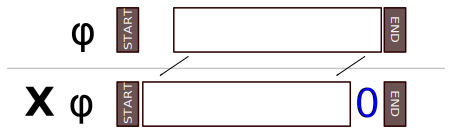
\includegraphics[scale=0.3]{Pattern-X}}~~~
\subfloat[$\mbox{\bf G}\,\varphi$]{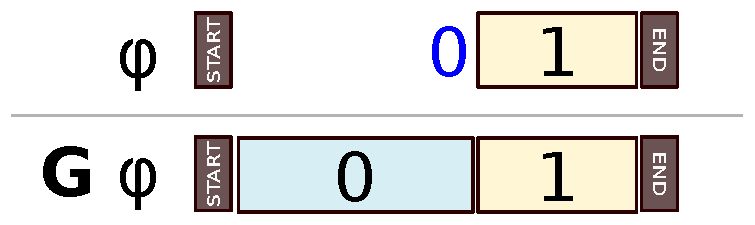
\includegraphics[scale=0.3]{Pattern-G}}~~~
\subfloat[$\varphi\,\mbox{\bf U}\,\psi$]{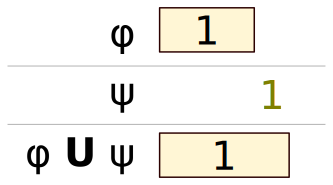
\includegraphics[scale=0.3]{Pattern-U}}
\caption{A graphical representation of the computation of three temporal operators on bitmaps}
\label{fig:patterns}
\end{figure}

\begin{algorithm}
\caption{Computing $\X a$}
\label{alg:next}
\begin{algorithmic}[1]
\Require Bitmap $a$
%\State // X(10101) $\Rightarrow$ (0101)
\State $out \gets$ removeFirstBit($a$)
\State addMany($out$, 0, 1)
\State \Return $out$
\end{algorithmic}
\end{algorithm}

To compute the vector for $\G\psi$, it suffices to find the smallest position $i$ such that all subsequent bits are 1. In $B_{\G\psi}$, all bits before $i$ are set to 0, and all bits after (and including) $i$ are set to 1. Thus to implement this operator using bitmaps, we need to do a search in the bitmap $B_{\psi}$ from back to front to find the last occurrence of the bit 0, as can be seen from Algorithm \ref{alg:global}. % and \ref{alg:future}.

Operator \textbf{F} (See Algorithm \ref{alg:future}) is the dual of \textbf{G}; its corresponding algorithm works in the same way as for \textbf{G}, swapping 0 and 1.

\begin{algorithm}
\caption{Computing $\G a$}
\label{alg:global}
\begin{algorithmic}[1]
\Require Bitmap $a$
\State $p \gets$ last(0, $a$)
\If {$p = -1$}
  \State \Return $a$
\Else
  \State $out \gets \langle~\rangle$
  \State addMany($out$, 0, $p + 1$)
  \State addMany($out$, 1, $|a| - p - 1$)
  \State \Return $out$
\EndIf
\end{algorithmic}
\end{algorithm}

\begin{algorithm}
\caption{\textbf{F}uture}
\label{alg:future}
\begin{algorithmic}[1]
\Require Bitmap $a$
%\State // F(010100) $\Rightarrow$ (111100)
\State $pos \gets$ last(1, $a$)
\If {$pos = -1$}
  \State \Return $a$
\Else
  \State $out \gets$ empty Bitmap
  \State addMany($out$, 1, $pos + 1$)
  \State addMany($out$, 0, $|a| - pos - 1$)
  \State \Return $out$
\EndIf
\end{algorithmic}
\end{algorithm}

According to Definition \eqref{eq:until}, if there is an index $j$ such that $\overline{s}^j \models \psi$ and $\overline{s}^i$ for all $i < j$, then $\overline{s}\models \varphi\U\psi$. In terms of bitmap operations, we need to keep checking if there is any bit set as 1 in $B_{\varphi}$ before every occurrence of bit 1 in $B_{\psi}$ (see Algorithm \ref{alg:until}).

\begin{algorithm}
\caption{Computing $a \U b$}
\label{alg:until}
\begin{multicols}{2}
\begin{algorithmic}[1]
\Require Bitmaps $a$ and $b$
\State $out \gets \langle~\rangle$
\State $p, a_0, a_1, b_0, b_1 \gets 0$
\While {$p < |a|$}
  \If {$a_1 \leq p$}
    \State $a_1 \gets$ next(1, $a$, $p$)
  \EndIf

  \If {$b_1 \leq p$}
    \State $b_1 \gets$ next(1, $b$, $p$)
  \EndIf

  \If {$a_1 = -1$ or $b_1 = -1$}
    \State \textbf{break}
  \EndIf

  \State $nearest1 \gets$ min($a_1$, $b_1$)
  \If {$nearest1 > p$}
    %\State // (00..) U (00..) $\Rightarrow$ (00..)
    \State addMany($out$, 0, $nearest1 - p$)
    \State $p \gets nearest1$
    \State \textbf{continue}
  \EndIf

  \If {$p = b_1$}
    %\State // (??..) U (11..) $\Rightarrow$ (11..)
    \If {$b_0 \leq b_1$}
      \State $b_0 \gets$ next(0, $b$, $b_1$)
      \If {$b_0 = -1$}
        \State $b_0 \gets |a|$
      \EndIf
    \EndIf
    \State addMany($out$, 1, $b_0 - p$)
    \State $p \gets b_0$
    \State \textbf{continue}
  \EndIf

  \If {$a_0 \leq a_1$}
    \State $a_0 \gets$ next(0, $a$, $a_1$)
    \If {$a_0 = -1$}
      \State $a_0 \gets |a|$
    \EndIf
  \EndIf
  \If {$a_0 \geq b_1$}
    %\State // (111?..) U (0001..) $\Rightarrow$ (1111..)
    \State addMany($out$, 1, $b_1 - p + 1$)
    \State $p \gets b_1 + 1$
  \Else
    %\State // (11100..) U (00001..) $\Rightarrow$ (00000..)
    \State addMany($out$, 0, $a_0 - p + 1$)
    \State $p \gets a_0 + 1$
  \EndIf
\EndWhile

\If {$b_1 = -1$}
  %\State // (..??) U (..00) $\Rightarrow$ (..00)
  \State addMany($out$, 0, $|a| - |out|$))
\ElsIf {$a_1 = -1$}
  %\State // (..0000) U (..1010) $\Rightarrow$ (..1010)
  \State copyTo($out$, $b$, $p$, $|a| - p$)
\EndIf

\State \Return $out$
\end{algorithmic}
  \end{multicols}
\end{algorithm}

The operation $\psi \textbf{ W } \varphi$ (Definition \eqref{eq:wuntil}) is quite like $\psi \textbf{ U } \varphi$, except that as the equation \eqref{eq:uw} \citep{huth2004} entails, the operation of the former also includes the operation $\textbf{G}\psi$. Algorithm \ref{alg:wuntil} explains its operation.

\begin{equation} \label{eq:uw}
\psi \textbf{W} \varphi \equiv \psi \textbf{U} \varphi \vee \textbf{G}\psi
\end{equation}

\begin{algorithm}
\caption{Computing $a \W b$}
\label{alg:wuntil}
\begin{multicols}{2}
\begin{algorithmic}[1]
\Require Bitmaps $a$ and $b$
\State $out \gets \langle~\rangle$
\State $p, a_0, a_1, b_0, b_1 \gets 0$
\While {p < |a|}
  \If {$a_1 \leq p$}
    \State $a_1 \gets$ next(1, $a$, $p$)
  \EndIf
  \If {$b_1 \leq p$}
    \State $b_1 \gets$ next(1, $b$, $p$)
  \EndIf
  \If {$a_1 = -1$ or $b_1 = -1$}
    \State \textbf{break}
  \EndIf

  \State $nearest1 \gets$ min($a_1$, $b_1$)
  \If {$nearest1 > p$}
    \State addMany($out$, 0, $nearest1 - p$)
    \State $p \gets nearest1$
    \State \textbf{continue}
  \EndIf

  \If {$p = b_1$}
    \If {$b_0 \leq b_1$}
      \State $b_0 \gets$ next(0, $b$, $b_1$)
      \If {$b_0 = -1$}
        \State $b_0 \gets |a|$
      \EndIf
    \EndIf
    \State addMany($out$, 1, $b_0 - p$)
    \State $p \gets b_0$
    \State \textbf{continue}
  \EndIf

  \If {$a_0 \leq a_1$}
    \State  $a_0 \gets$ next(0, $a$, $a_1$)
    \If {$a_0 = -1$}
      \State $a_0 \gets |a|$
    \EndIf
  \EndIf

  \If {$a_0 \geq b_1$}
    \State addMany($out$, 1, $b_1 - p + 1$)
    \State $p \gets b_1 + 1$
  \Else
    \State addMany($out$, 0, $a_0 - p + 1$)
    \State $p \gets a_0 + 1$
  \EndIf
\EndWhile

\If {$b_1 = -1$}
  \If {$a_1 = -1$}
    \State addMany($out$, 0, $|a| - |out|$)
  \Else
    \State $last0 \gets$ last(0, $a$)
    \If {$last0 = -1$ or $last0 < p$}
      \State addMany($out$, 1, $|a| - |out|$)
    \Else
      \State addMany($out$, 0, $last0 - p + 1$)
      \State addMany($out$, 1, $|a| - |out|$)
    \EndIf
  \EndIf
\ElsIf {$a_1 = -1$}
  \State copyTo($out$, $b$, $|b| - b_1 - 1$, $|b| - b_1$)
\EndIf

\State \Return $out$
\end{algorithmic}
\end{multicols}
\end{algorithm}

As the dual of the operator \textbf{U}, the operator \textbf{R} defined in \eqref{eq:release} need to union two parts for the formula $\psi \textbf{R} \varphi$: the first part aims to find whether exist $i, j (0 \leq i < j)$ which make $\pi^i, \pi^{i + 1}, ... \pi^j$ satisfy $\varphi$ when $\pi^j$ satisfies $\psi$; and the second is simply $G\varphi$. Algorithm \ref{alg:release} describes this procedure.

\begin{algorithm}
\caption{Computing $a \R b$}
\label{alg:release}
\begin{multicols}{2}
\begin{algorithmic}[1]
\Require Bitmaps $a$ and $b$
\State $out \gets \langle~\rangle$
\State $p, a_0, a_1, b_0, b_1 \gets 0$
\While {$p < |a|$}
  \If {$b_1 \leq p$}
    \State $b_1 \gets$ next(1, $b$, $p$)
  \EndIf
  \If {$b_1 = -1$}
    \State \textbf{break}
  \EndIf

  \If {$b_1 > p$}
    \State addMany($out$, 0, $b_1 - p$)
    \State $p \gets b_1$
    \State \textbf{continue}
  \EndIf

  \If {$a_1 \leq p$}
    \State $a_1 \gets$ next(1, $a$, $p$)
  \EndIf
  \If {$a_1 = -1$}
    \State \textbf{break}
  \EndIf

  \If {$b_0 \leq b_1$}
    \State $b_0 \gets$ next(0, $b$, $b_1$)
    \If {$b_0 = -1$}
      \State $b_0 \gets |a|$
    \EndIf
  \EndIf
  \If {$a_1 \geq b_0$}
    \State addMany($out$, 0, $b_0 - p + 1$)
    \State $p \gets b_0 + 1$
    \State \textbf{continue}
  \EndIf

  \If {$a_0 \leq a_1$}
    \State $a_0 \gets$ next(0, $b$, $a_1$)
    \If {$a_0 = -1$}
      \State $a_0 \gets |a|$
    \EndIf
  \EndIf
  \State $nearest0 \gets$ min($a_0$, $b_0$)
  \State addMany($out$, 1, $nearest0 - p$)
  \State $p \gets nearest0$
\EndWhile

\If {$a_1 = -1$ and $b_1 \neq -1$}
  \State $last0 \gets$ last(0, $b$)
  \If {$last0 = -1$ and $last0 < p$}
    \State addMany($out$, 1, $|a| - |out|$)
  \Else
    \State addMany($out$, 0, $last0 - p + 1$)
    \State addMany($out$, 1, $|a| - |out$)
  \EndIf
\Else
  \State addMany($out$, 0, $|a| - |out|$)
\EndIf

\State \Return $out$
\end{algorithmic}
\end{multicols}
\end{algorithm}

\subsection{Discussion}

An interesting point of this last algorithm is that the bitmaps $a$ and $b$ are not traversed in a linear fashion. Rather, entire blocks of each bitmap can be skipped to reach directly the next 0 or the next 1, depending on the case. Note that this is only possible if the trace is completely known in advance before starting to evaluate a formula (and moreover, the trace is traversed backwards). Therefore, our proposed solution is an example of an offline monitor that is not simply an online monitor that is fed events of a pre-recorded trace one by one: it exploits the possibility of \emph{random access} to parts of the trace that is only possible in an offline setting.

This example shows one of the advantages of our proposed technique in terms of complexity. Indeed, reading the original log to create the ground bitmaps can be done in linear time (and in a single pass for all propositional symbols at once). However, once these initial bitmaps are computed, many of the required operations do not require a linear processing of the trace anymore. For example, evaluating $\X\varphi$ requires a simple bit shift, which can be done in a single CPU operation for 64 bits at a time, and potentially much more if compression is used.\footnote{The left bit shift of a compressed block is the block itself, as long as the next bit to the right has the same value.} Similarly, looking for the next 0 or 1 seldom requires linear searching, as the use of compression makes it possible to skip over fill words in one operation. Computing the bitmap for a \textbf{F} or \textbf{G} operator requires a single such lookup for the entire trace.

Another interesting point is the fact that operators \textbf{F} and \textbf{G} are monotonous. As can be seen in Figure \ref{fig:patterns}, the resulting bitmap is of the form $0^*1^*$ (or the reverse). Hence a very simple bitmap is propagated upwards to further algorithms; it can be heavily compressed, and makes any lookup for the next 0 or the next 1 trivial. While not producing such simple vectors, bitmaps resulting from the application of \textbf{U} still have a relatively regular structure that is again amenable to reasonable compression.

%% }}} --- Subsection

%% }}} --- Section

%% ------------------
%% Section: expériences
%% ------------------
\section{Implementation and Experiments}\label{sec:bm:experiments} %% {{{

While the worst-case complexity of every algorithm presented in the previous section is still $O(n)$ (where $n$ is the size of the input bitmap), we suspect that performance in practice should be much better. Therefore, in this section, we describe experiments in order to achieve the following purposes:

\begin{enumerate}
\item Test the performance of fundamental LTL algorithms
\item Test the performance of the recursive application of these algorithms on complex LTL formul\ae{}
\item Evaluate the performance and space savings incurred by the use of compression
\end{enumerate}

\begin{comment}
\subsection{Modifications to Libraries} %% {{{

Section \ref{sec:bm:ltlbitmap} mentions that the time and space complexities of all LTL operators are $O(n)$ where $n$ is the size of the input uncompressed bitmap. After applying RLE-model bitmap compression algorithms to our solution, the space complexities become $O(m)$ as is discussed above, and we managed to make the time complexities also become $O(m)$ by implementing the bitmap manipulation functions listed in Table \ref{tbl:bm:bmhelpers} for every  bitmap compression algorithms.

Because of lack of the support of random access for the RLE-model bitmap compression algorithms, we cannot enumerate the bits in the same way as uncompressed bitmap. Therefore we design an \emph{iterator} data structure to store not only the absolute index of current bit in the uncompressed bitmap but also the relative index in the compressed bitmap.

Taking the function \textbf{next(1, )} as an example, if the current relative index is in a sequence word of 0, the search in this word is unnecessary, and we just jump to the next word; if the index is in a sequence word of 1, we return the current index; however, if the index is in a literal word, we have to look for the bit 1 in the $ulen$-bits word.

%% }}}
\end{comment}

\subsection{Experimental Setup} %% {{{

As a means to avoid the runtime disk I/O cost we load all relevant files into memory before the calculations. Thus although using bitmap can considerably reduce the requirement of memory, we prepared a workstation with an Intel Xeon E5-2630 v3 Processor and 48 GB of memory.

All codes are implemented in Java which self takes responsibility of the memory management and garbage collection. Concerning the delay caused by garbage collection (GC) and especially Full-GC, we called \textit{System.gc()} before and after every formula calculation to provide a runtime environment that was as ``clean'' as possible.

Table \ref{table:bmlibs} shows the libraries used for different types of bitmap. In order to implement all the LTL operations, we modified the codes of the libraries to add the necessary functions listed in Table \ref{tbl:bm:bmhelpers} and to optimize the functions so that the time complexities of the operators become $O(m)$ where $m$ is the number of sequences of consecutive 0/1 bits.

\begin{table}
\centering
\begin{tabular}{|c|l|}
\hline
Bitmap & Source \\
\hline
Uncompressed & \texttt{java.util.BitSet} from Java SDK \\
\hline
\multirow{2}{*}{WAH} & Original:\ \ \url{https://github.com/metamx/extendedset} \\
& Modified: \url{https://github.com/phoenixxie/extendedset} \\
\hline
\multirow{2}{*}{Concise} & Original:\ \ \url{https://github.com/metamx/extendedset} \\
& Modified: \url{https://github.com/phoenixxie/extendedset} \\
\hline
\multirow{2}{*}{EWAH} & Original:\ \ \url{https://github.com/lemire/javaewah} \\
& Modified: \url{https://github.com/phoenixxie/javaewah} \\
\hline
Roaring & \url{https://github.com/lemire/RoaringBitmap} \\
\hline
\end{tabular}
\caption{Bitmap libraries}
\label{table:bmlibs}
\end{table}

Because of lack of the support of random access for the RLE-model bitmap compression algorithms, we cannot enumerate the bits in the same way as for an uncompressed bitmap. Therefore we designed an \emph{iterator} data structure to store not only the absolute index of current bit in the uncompressed bitmap but also the relative index in the compressed bitmap. Taking the function \textbf{next(1,x)} as an example, if the current relative index is in a sequence word of 0, the search in this word is unnecessary, and we just jump to the next word; if the index is in a sequence word of 1, we return the current index; however, if the index is in a literal word, we have to look for the bit 1 in the $ulen$-bits word.

For the experiments, we developed a random data generator. Every time it generates $5 \times 10^7$ tuples, and each tuple contains 3 random numbers ($a, b, c$) related with 3 simple inequalities: $a > 0$, $b > 0$ and $c \leq 0$, which will be labelled as $s_0$, $s_1$ and $s_2$, respectively. According to \eqref{eq:ap}, the true/false values of these 3 statements consist of the atomic propositions. When a tuple was passed to the 3 statements, we got 3 boolean values each of which was then turned into a 1/0 bit in the bitmap corresponding to one of the 3 statements. When all tuples were processed, we had 3 bitmaps having 50 million bits each.

% The experiment data was a file with 50 million lines of states, each of which contained 3 random numbers used for 3 relational statements. The true/false values of these 3 statements $(s_0, s_1, s_2)$ consisted of the atomic propositions.

% \begin{table}
% \centering
% \begin{tabular}{|c|c|}
% \hline
% & Relational statement \\
% \hline
% $s_0$ & $a > 0$ \\
% \hline
% $s_1$ & $b > 0$ \\
% \hline
% $s_2$ & $c \leq 0$ \\
% \hline
% \end{tabular}
% \caption{Relational statements}
% \label{tbl:bm:statements}
% \end{table}

% Pas vraiment pertinent --SH
% The range of the random numbers is [-10000, 10000], and according to the three inequalities mentioned earlier, it is easy to know that the difference between the probabilities of getting 1 and getting 0 is only about $0.05\permil$ if the random function is fair enough, therefore there should be nearly the same number of 1 and 0 bits in the generated bitmap.

\subsection{Basic LTL Operators} %% {{{

A first experiment consisted of evaluating the performance, in terms of computation time, for evaluating a bit vector on each propositional and temporal operator taken separately.

In the first experiment, we ran 100 passes of a benchmark on the fundamental operators with uncompressed bitmaps. In every pass, the experiment data was regenerated and passed to the relational statements from which the bitmaps were created. Then the formul\ae{} were executed with the bitmaps. In the final step we calculated the average running time of a pass for each LTL operator, and the number of bits processed per second.

Table \ref{tbl:bm:basicops} shows that the propositional logic operators were faster than most temporal logic operators. Among the temporal logic operators, the binary operators were slower than the unary ones because the former require more operations than the latter, especially in the situation that many 0s and 1s sequences are mixed in the bitmap. The dual operators \textbf{G} and \textbf{F} have similar algorithms but \textbf{F} surprisingly took three times longer than \textbf{G}. This can be explained by the fact that for a fairly-randomized input bitmap, \textbf{F} will append more 1s than 0s to its output bitmap, while \textbf{G} will append more 0s than 1s. Although the Java \texttt{BitSet} implementation supports both to set a bit to 1 and to clear a bit to 0\footnote{\url{https://docs.oracle.com/javase/8/docs/api/java/util/BitSet.html}}, it actually does nothing when clearing a new bit of which the index is beyond its size, i.e. appending a bit 0. This results in an asymmetrical processing of 0s and 1s in the bitmap.

\begin{table}
\centering
\small
\begin{tabular}{|c|c|c|c|c|}
\hline
Formula & Min.\ time & Max.\ time & Avg.\ time & Throughput \\
& (ms) & (ms) & (ms) & (b/s) \\
\hline
$\neg s_0$ & 0 & 15 & 6.18 & $8.09 \times 10^{9}$ \\
\hline
$s_0 \wedge s_1$ & 0 & 16 & 5.86 & $8.53 \times 10^{9}$ \\
\hline
$s_0 \vee s_1$ & 0 & 16 & 5.8 & $8.62 \times 10^{9}$ \\
\hline
$s_0 \rightarrow s_1$ & 0 & 16 & 4.66 & $1.07 \times 10^{10}$ \\
\hline
$\X s_0$ & 0 & 16 & 8.93 & $5.60 \times 10^{9}$ \\
\hline
$\G s_0$ & 46 & 63 & 51.3 & $9.75 \times 10^8$ \\
\hline
$\F s_0$ & 140 & 174 & 150.55 & $3.32 \times 10^8$ \\
\hline
$s_0 \U s_1$ & 1562 & 2017 & 1747.05 & $5.72 \times 10^7$ \\
\hline
$s_0 \W s_1$ & 1531 & 1957 & 1685.71 & $5.93 \times 10^7$ \\
\hline
$s_0 \R s_1$ & 1735 & 2188 & 1961.37 & $5.10 \times 10^7$ \\
\hline
\end{tabular}
\vskip 8pt
\caption{Running time for evaluating each LTL operator on a bit vector, without the use of a compression library.}
\label{tbl:bm:basicops}
\end{table}

%% }}} --- Subsection

\subsection{Complex formul\ae{}} %% {{{

The results from this first experiment suggest that propositional logic operators, temporal logic unary operators and temporal logic binary operators have different magnitudes of processing speed; therefore we can divide the operators into three groups.

At the beginning of this second experiment, we composed various combinations of operators into 14 LTL formul\ae{} with the help of the tool \emph{randltl} from the library \textit{Spot} \footnote{\url{https://spot.lrde.epita.fr/index.html}}; the formul\ae{} are shown in Table \ref{tbl:bm:complex-formulas}. Then we also ran a 50-pass benchmark on the these formul\ae{} with uncompressed bitmaps. In each cycle the data was regenerated and re-executed with the 14 formul\ae{}. We measured the running time of each cycles and calculated the average time cost and the processing speed as before.


\begin{table}[h]
%\begin{footnotesize}

\begin{equation}\tag{F1}
\G ((s_2 \mathrel{\rightarrow} \F (\mathop{\neg}(s_1 \U  s_2) \W  (s_2 \mathrel{\vee} \G s_1))) \W  (\mathop{\neg}\F (s_0 \R  \X s_2) \W  ((s_0 \mathrel{\wedge} s_2 \mathrel{\wedge} \F s_2) \U  s_0)))
\end{equation}
%
\squeeze
%
\begin{equation}\tag{F2}
\F (\mathop{\neg}(s_2 \mathrel{\rightarrow} \X (s_0 \U  s_1)) \U  (\mathop{\neg}(s_0 \mathrel{\vee} \F \X (s_0 \U  (\X (\F s_1 \W  s_1) \R  s_1))) 
\U  (s_0 \R  \G s_2)))
\end{equation}
%
\squeeze
%
\begin{equation}\tag{F3}
\X \F ((s_1 \mathrel{\vee} s_2 \mathrel{\vee} (\G (s_0 \mathrel{\vee} s_1 \mathrel{\vee} \mathop{\neg}s_1) \mathrel{\wedge} \X \mathop{\neg}s_0)) \mathrel{\rightarrow} \\
((\mathop{\neg}s_0 \mathrel{\rightarrow} (s_0 \mathrel{\wedge} \mathop{\neg}s_1)) \mathrel{\wedge} \G s_0))
\end{equation}
%
\squeeze
%
\begin{equation}\tag{F4}
\X (\mathop{\neg}\G (s_0 \mathrel{\rightarrow} s_2) \mathrel{\rightarrow} \F (s_1 \mathrel{\wedge} ((\F (s_0 \mathrel{\wedge} s_2) \mathrel{\rightarrow} s_1) \mathrel{\rightarrow} \X \mathop{\neg}s_2) \mathrel{\wedge} \G (s_2 \mathrel{\rightarrow} (s_2 \mathrel{\wedge} \F s_1))))
\end{equation}
%
\squeezemore
%
\begin{multline}\tag{F5}
\mathop{\neg}((s_0 \U  (\mathop{\neg}(\mathop{\neg}s_0 \mathrel{\wedge} s_2) \mathrel{\vee} (\mathop{\neg}s_0 \W  (s_2 \mathrel{\rightarrow} s_0)))) \\
\W  \mathop{\neg}s_0) \mathrel{\vee}
(s_1 \R  ((s_1 \mathrel{\vee} (s_0 \W  s_2)) \W  (\mathop{\neg}s_0 \W  s_2)))
\end{multline}
%
\squeeze
%
\begin{equation}\tag{F6}
(s_1 \W  ((s_2 \mathrel{\rightarrow} (\mathop{\neg}s_2 \R  \mathop{\neg}(\mathop{\neg}s_1 \W  s_0))) \W  (\mathop{\neg}s_1 \mathrel{\vee} \mathop{\neg}((\mathop{\neg}s_2 \mathrel{\rightarrow} s_1) \mathrel{\rightarrow} \mathop{\neg}s_0)))) \W  (s_0 \R  \mathop{\neg}s_2)
\end{equation}
%
\squeezemore
%
\begin{multline}\tag{F7}
\X (((\F s_2 \R  s_0) \U  \F s_0) \R  \G ((s_2 \W  s_1) \W  \\
(((\G s_2 \U  s_1) \R  \X s_0) \R  (s_2 \W  ((s_2 \R  \X s_2) \W  s_1)))))
\end{multline}
%
\squeezemore
%
\begin{equation}\tag{F8}
(\G (s_0 \R  \F s_1) \U  \F s_2) \W  \G ((s_1 \U  s_2) \R  ((\G \X s_0 \U  (s_2 \W  s_0)) \W  \F ((\G s_1 \U  s_2) \R  s_2)))
\end{equation}
%
\squeeze
%
\begin{equation}\tag{F9}
\G \F (\G \F s_0 \mathrel{\wedge} \F \X \G s_1 \mathrel{\wedge} \G \F \X \X \X \G \X \F \G s_2)
\end{equation}
%
\squeeze
%
\begin{equation}\tag{F10}
\F \G \F \X (\X s_2 \mathrel{\wedge} \X \G \X \X \G \F (\G \X \F s_1 \mathrel{\wedge} \X \G s_0))
\end{equation}
%
\squeeze
%
\begin{equation}\tag{F11}
\mathop{\neg}(((s_0 \mathrel{\vee} s_2) \mathrel{\rightarrow} (\mathop{\neg}(s_2 \mathrel{\wedge} (\mathop{\neg}s_2 \mathrel{\rightarrow} \mathop{\neg}(s_0 \mathrel{\wedge} (s_0 \mathrel{\vee} \mathop{\neg}s_1)))) \mathrel{\vee} (s_0 \mathrel{\wedge} \mathop{\neg}s_0))) \mathrel{\vee} (\mathop{\neg}s_0 \mathrel{\wedge} (s_0 \mathrel{\vee} s_2)))
\end{equation}
%
\squeezemore
%
\begin{multline}\tag{F12}
(s_1 \mathrel{\wedge} \mathop{\neg}s_2 \mathrel{\wedge} (s_2 \mathrel{\rightarrow} s_0)) \mathrel{\vee} \mathop{\neg}((s_0 \mathrel{\wedge} \mathop{\neg}s_0) \mathrel{\rightarrow} s_1) \mathrel{\vee} \\
((s_2 \mathrel{\vee} (s_1 \mathrel{\rightarrow} s_0)) \mathrel{\wedge} ((s_0 \mathrel{\wedge} \mathop{\neg}s_2 \mathrel{\wedge} (s_1 \mathrel{\rightarrow} s_0)) \mathrel{\rightarrow} s_0))
\end{multline}
%
\squeezemore
%
\begin{multline}\tag{F13}
(((s_0 \W  s_2) \W  s_0) \U  ((s_1 \U  (((s_1 \W  s_2) \W  (s_1 \R  (s_1 \R  s_0))) \W  s_2)) \W  s_2)) \W  \\
((s_0 \R  s_1) \R  (((s_2 \U  s_1) \U  s_1) \R  ((s_0 \W  s_2) \W  s_1)))
\end{multline}
%
\squeezemore
%
\begin{multline}\tag{F14}
((((s_1 \U  s_2) \U  (s_2 \U  s_1)) \U  s_1) \R  (s_1 \R  s_2)) \U  (((s_2 \W  ((s_0 \W  \\
((s_2 \R  s_0) \R  s_1)) \U  s_1)) \W  s_0) \W  (((s_0 \R  s_1) \R  (s_0 \W  s_1)) \U  s_0))
\end{multline}

%\end{footnotesize}
\vskip 8pt
\caption{The complex LTL formul\ae{} evaluated experimentally.}
\label{tbl:bm:complex-formulas}
\end{table}

As is indicated in Table \ref{tbl:bm:complex}, 3 groups of operators have different scales of processing speed. The combinations having temporal logic and binary operators always took more time than others, and formul\ae{} 13 and 14 are the slowest. This result also shows that our solution can handle a fairly large number of bits (events from the trace) per second, ranging from millions to billions.

\begin{table}[h]
\centering
\small
\begin{tabular}{|c|c|c|c|c|c|c|c|}
\hline
Formula & Prop. & Temp. & Temp. & Min Time & Max Time & Avg. Time & Approx. \\
No. & Logic & Unary & Binary & (ms) & (ms) & (ms) & bits/second \\
& Ops. & Ops. & Ops. & & & & \\
\hline
F1 & 6 & 6 & 6 & 10454 & 14205 & 11483.02 & $1.31 \times 10^7$ \\
\hline
F2 & 4 & 7 & 7 & 7728 & 10673 & 8937.59 & $1.68 \times 10^7$  \\
\hline
F3 & 13 & 5 & 0 & 281 & 422 & 326.63 & $4.59 \times 10^8$  \\
\hline
F4 & 11 & 7 & 0 & 422 & 704 & 560.58 & $2.68 \times 10^8$  \\
\hline
F5 & 11 & 0 & 7 & 8532 & 10496 & 9374.5 & $1.60 \times 10^7$  \\
\hline
F6 & 12 & 0 & 6 & 7280 & 9357 & 7934.6 & $1.89 \times 10^7$  \\
\hline
F7 & 0 & 7 & 11 & 12330 & 15004 & 13413.91 & $1.18 \times 10^7$  \\
\hline
F8 & 0 & 8 & 10 & 9442 & 11833 & 10428.37 & $1.44 \times 10^7$  \\
\hline
F9 & 2 & 16 & 0 & 431 & 1155 & 682.68 & $2.20 \times 10^8$  \\
\hline
F10 & 2 & 16 & 0 & 375 & 857 & 472.76 & $3.17 \times 10^8$  \\
\hline
F11 & 18 & 0 & 0 & 31 & 56 & 45.18 & $3.32 \times 10^9$  \\
\hline
F12 & 18 & 0 & 0 & 46 & 68 & 51.58 & $2.91 \times 10^9$  \\
\hline
F13 & 0 & 0 & 18 & 22768 & 27308 & 24825.21 & $6.04 \times 10^6$  \\
\hline
F14 & 0 & 0 & 18 & 22800 & 27481 & 24877.67 & $6.03 \times 10^6$  \\
\hline
\end{tabular}
\vskip 8pt
\caption{Running time for the evaluation of LTL formul\ae{} of Table \ref{tbl:bm:complex-formulas}, without the use of a compression library.}
\label{tbl:bm:complex}
\end{table}

%% }}} --- Subsection

\subsection{Use of Bitmap Compression} %% {{{

According to the RLE-model algorithms, the compression ratio mostly depends on the length of consecutive 0s or 1s. Hence in this experiment we modified the generator to enable it to repeat the same tuple a specified number of times: 1, 32 and 64. This new mechanism is able to ensure the existence of continuous sequences with a minimum length ($slen$) in the generated bitmaps. Intuitively, when the value of $slen$ increases, the number of sequences decreases; therefore the RLE-model algorithms can be expected to have better performance than an uncompressed bitmap. % for its $O(m)$ time and space complexities.

\begin{figure}[h]
\begin{center}
\centering
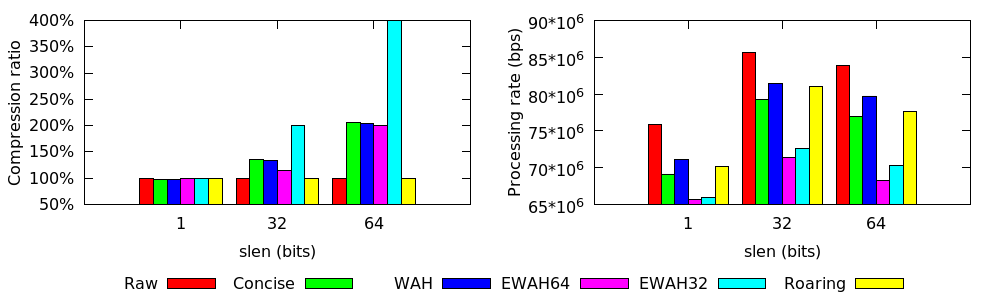
\includegraphics[width=\linewidth]{states.png}
\caption{Bitmap generation with compression algorithms}
\label{img:states}
\end{center}
\end{figure}

In the first part of the experiment, we generated the bitmaps with different algorithms and different values of $slen$, and then calculated the compression ratios. The result in Figure \ref{img:states} confirms the hypothesis that when $slen < wlen$ (where $wlen$ is the length of a word), the bitmap cannot be well compressed by any RLE-model algorithm, and in this case, the algorithm EWAH behaves a little better than the others due to its smaller structural cost. When $slen$ increases to 32 and 64, i.e. $slen \geq wlen$, the RLE algorithms start to work well and the compression ratio of $slen = 64$ is obviously better than the one of $slen = 32$. From the figure \ref{img:states} we can also see that when $slen$ is 1, 32 and 64, EWAHs are much slower than WAH, Concise and Roaring.

\begin{comment}
The result in Figure \ref{img:ratio} shows that when the length of consecutive bits is small ($\leq 5$), there is no great gap of the ratio among the RLE-model algorithms, Roaring bitmap and even uncompressed bitmap. The word lengths of WAH, Concise, EWAH(32bit), EWAH(64bit) are 32, 32, 32 and 64, so when the length grows beyond 50, which is over 32 and slightly less than 64, the ratios increase dramatically. The compression ratio of Roaring bitmap depends on the fraction of 1s bits in the bitmap, when the bitmap is not very sparse, the algorithm has to allocate much memory for its containers which in our opinion is the reason that its compression ratio is near 1 (uncompressed).
\end{comment}

In the second part of the experiment, we measured the performance of the compressed bitmaps when applying the algorithms for all fundamental operators and all LTL formul\ae{}s in the previous experiments. Detailed results covering all the operators and formul\ae{}s can be found in Appendix \ref{appendixa}.

To this end, we picked formula F1 and F14 from the previous experiment, as F1 contains all the operators and connectives of LTL and F14 is the slowest of all formul\ae{} in the previous experiment. We again ran the benchmark 100 passes; in each cycle, the formula was evaluated with one group of input bitmaps from the last step and we recorded the time cost of each bitmap algorithm and each length of consecutive bits.

\begin{figure}[h]
\begin{center}
\centering
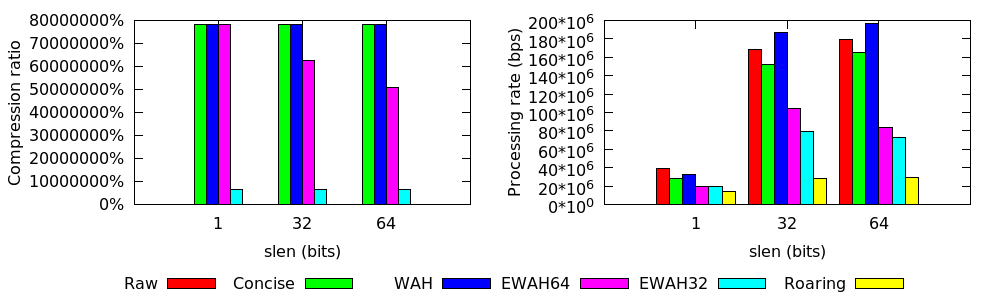
\includegraphics[width=\linewidth]{p11.png}
\caption{Comparison of compression ratio and processing rate for LTL formula 1, for various bitmap compression libraries and various values of $slen$}
\label{img:f1}
\end{center}
\end{figure}

\begin{figure}[h]
\begin{center}
\centering
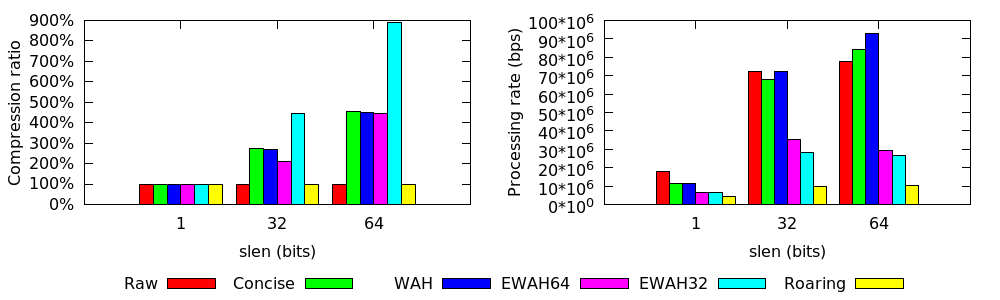
\includegraphics[width=\linewidth]{p24.png}
\caption{Comparison of compression ratio and processing rate for LTL formula 14, for various bitmap compression libraries and various values of $slen$}
\label{img:f14}
\end{center}
\end{figure}

According to Figure \ref{img:f1} and \ref{img:f14}, the performance of the RLE-model algorithms, WAH, EWAH and Concise is obviously related to the value of $slen$. The Figure \ref{img:f1} also suggests that the presence of operators \textbf{G} and \textbf{F} can vastly increase the length of consecutive bits of same value, which in turn can be well compressed by RLE-model algorithms. In such a case, several algorithms have better performance than the uncompressed bitmap as $slen$ increases.

%% }}} --- Subsection

%% }}} --- Section

%% ------------------
%% Section: related work
%% ------------------
\section{Related Work}\label{sec:bm:related} %% {{{

The prospect of using physical properties of hardware to boost the performance of runtime verification has already been studied in the recent past. For example, Pellizzoni \etal\@ \citep{pellizzoni2008hardware} utilized dedicated commercial-off-the-shelf (COTS) hardware \citep{emerson1990temporal} to facilitate the runtime monitoring of critical embedded systems whose properties were expressed in Past-time Temporal Linear Logic (PTLTL).

As the number of cores (GPU or multi-core CPUs) in the commodity hardware keeps increasing, the research of exploiting the available processors or cores to parallelize the tasks and the computing  brings a challenge and also an opportunity to improve the architecture of runtime verification. For example, Ha \etal\@ \citep{ha2009concurrent} introduced a buffering design of \emph{Cache-friendly Asymmetric Buffering (CAB)} to improve the communications between application and runtime monitor by exploiting the shared cache of the mutilcore architecture; Berkovich \etal\@ \citep{DBLP:journals/fmsd/BerkovichBF15} proposed a GPU-based solution that effectively utilizes the available cores of the GPU, so that the monitor designed and implemented with their method can run in parallel with the target program and evaluate LTL properties.

Previous work by one of the authors \citep{jocasa} introduced an algorithm for the automated verification of Linear Temporal Logic formul\ae{} on event traces, using an increasingly popular cloud computing framework called MapReduce. The algorithm can process multiple, arbitrary fragments of the trace in parallel, and compute its final result through a cycle of runs of MapReduce instances.
The proposed technique manipulates objects called \emph{tuples}, which are of the form $\langle \phi, (n, i)\rangle$, and are interpreted as the statement ``the process is at iteration $i$, and LTL formula $\phi$ is true for the suffix of the current trace starting at its $n$-th event''. One can see that this statement corresponds exactly to the fact, in the present solution, that the $n$-th position of the bitmap generated by the evaluation of $\phi$ contains the value 1.

Apart from this similarity, however, the two techniques are radically different. Since the MapReduce approach operates on tuples one by one, while the present solution manipulates entire bitmaps, the algorithms for each LTL operator have little in common (especially that for \textbf{U}). Where the MapReduce approach gets its speed from the processing of multiple subformul\ae{} on different machines, our present solution is efficient because some operations (such as conjunction) can be computed simultaneously for many adjacent events in a single CPU cycle. In addition, a downside of the MapReduce solution is the large number of tuples generated, and the impossibility of compressing that volume of data.

As one can see, there have been multiple attempts at leveraging parallelism and properties of hardware to evaluate temporal expressions on traces. However, As far as we know, our work it the first to get its performance boost at the level of the \emph{data structures} used to evaluate these expressions.

%% }}} --- Section

%% ------------------
%% Section: conclusion
%% ------------------
\section{Conclusion and future work}\label{sec:bm:conclusion} %% {{{

We proposed a solution for the offline evaluation of LTL formul\ae{} by means of bitmap manipulations. In such a setting, propositional predicates on individual events of a trace states are mapped to bits of a vector (``bitmap'') that are then manipulated to implement each LTL operator. In addition to the fact that bitmap manipulations are in themselves very efficient, our algorithms take advantage of the fact that the trace is completely known in advance, and that random access to any position of that trace makes it possible to skip large blocks of events to speed up the evaluation.

For this reason, our solution is a prime example of an offline evaluation algorithm that exploits the fact that it indeed works offline ---it is not merely an online algorithm that reads events from a pre-recorded trace one by one. As a matter of fact, in some cases (such as the \textbf{U} operator), the trace is even evaluated from the end, rather than from the beginning. A thorough performance benchmark for both fundamental operators and complex LTL formul\ae{} proved the feasibility of the approach, and showed how events from a trace can be processed at a rate ranging from millions to billions of events per second.

To further exploit the potential of bitmaps, we introduced bitmap compression algorithms in our solution and integrated them in our benchmark. In the experiments, as we expected, compressed bitmaps demonstrated thair ability to easily compress sparse bitmaps and accelerating the LTL operations when there is a certain amount of consecutive bits with the same value. We have explained, how many LTL operators naturally increase the regularity of the bitmaps they are processing.

Obviously, this solution is suitable only for offline evaluation. However, The promising results obtained in our implementation lead to a number of potential extensions and improvements over the current method. First, the algorithm can be reused as a basis for other temporal languages that intersect with LTL, such as PSL \cite{IntroPSLBook}. Second, the technique could be expanded to take into account data parameters and quantification. Finally, one could also consider to parallellize the evaluation of large segments of btimaps on multiple machines.

%% }}} --- Section

%% :folding=explicit:wrap=soft:mode=latex:
